\chapter{轨迹替换方法}

\section{工作原理}
在Gym环境中进行初步实验时,与\ref{HERsec}中的替换方法不同,不在采样时对已完成的目标进行替换,而是在将新的迁移保存到重放缓冲中时对整个片段进行进行替换,并把未替换和替换后的轨迹都加入到重放缓冲中。
换句话说,每当一个片段结束时,对这个片段中由所有迁移构成的整个轨迹中的已完成的目标进行替换,并把替换后的一整个新轨迹添加到原轨迹之后。

形式化地,轨迹替换会从重放缓冲中取出一整个轨迹的副本$s[1:T]=(o[1:T], g^a[1:T], g^d[1:T])$,并对其做如下替换:
$$g^d[1:T]=g^a[-1]$$
$$r[1:T]=reward(g^d[1:T], g^a[1:T])$$
并将所替换后的轨迹添加到重放缓冲中。

实验在\ref{gymexp}中设计的系统中进行,使用的实验参数见表\ref{pretable}。
    \begin{table}[htbp]
        \caption{初步实验参数}
        \label{pretable}
    \vspace{0.5em}\centering\wuhao
    \begin{tabular}{ccccc}
    \toprule[1.5pt]
    实验参数 & 值\\
    \midrule[1pt]
        $\epsilon_{noise}$ & 0.2\\
        $\sigma_{clip}$ & 0.5\\
        $M$ & 5120\\
        $\epsilon_{rand}$ & 0.3\\
        $\gamma$ & 0.99\\
        $\alpha$ & $3\times 10^{-4}$\\
        $B$ & 8\\
        $\tau$ & 0.005\\
        $T$ & 50\\
        $f_\mu$ & 2\\
        $T_{start}$ & $2.5\times 10^4$\\
        $N_{sample}$ & 10 \\
    \bottomrule[1.5pt]
    \end{tabular}
    \end{table}
    其中$\epsilon_{noise}$是在更新评论家网络权重,使用靶演员网络计算动作向量时添加进去的高斯噪声的标准差,$\sigma_{clip}$是对此噪声进行裁剪的阈值,裁剪后有噪声大小在区间$[-\sigma_{clip},\sigma_{clip}]$以内。
    $M$是重放缓冲能保存的迁移的最多数量。
    $\epsilon_{rand}$是采用$\epsilon$-greedy探索方法进行探索时,随机采样动作的概率大小。
    $\gamma$是前述折扣系数。
    $\alpha$是演员网络和评论家网络的优化器的学习率。
    $B$是从重放缓存中采样迁移的批次大小。
    $\tau$是\ref{td3sec}中所述的指数滑动平均系数。
    $T$是每个片段的最大时间步数。
    每经过$f_\mu$个时间步,才对演员网络权重进行更新一次,而评论家网络每权重更新和对靶网络权重的指数滑动平均更新在每个时间步都要做。
    在$t<T_{start}$时,使用完全随机的采样来得到智能体要做的动作,在$t\geq T_{start}$时,才开始使用演员网络获取动作向量。
    每经过$N_{sample}$个片段记为一代(epoch),对损失、奖励和成功率进行统计,最后绘制关于代的曲线图。

\section{实验结果}

        \begin{figure}
        \centering
        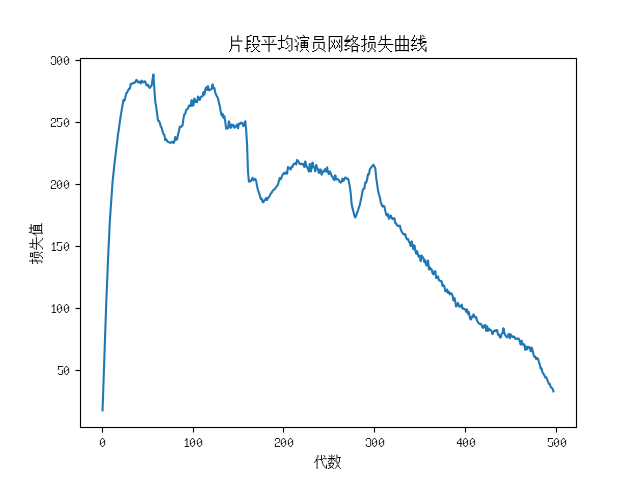
\includegraphics[width=0.6\textwidth]{mujoco_lossmu.png}
        \caption{$\mu$的损失曲线}
            \label{mujocolossmu}
        \end{figure}

        如图\ref{mujocolossmu}所示,演员网络在每个片段的平均损失在前60代快速上升,并在之后有回跳地下降。

        评论家网络1和评论家网络2的每个片段的平均损失如图\ref{mujocolossq1}和\ref{mujocolossq2}。
        通过对比可以看出两个图中的损失曲线的变化趋势大致相同且剧烈变化之处与演员网络的损失相似,这可能是由于评论家网络的好坏通过损失影响了演员网络表示的确定性策略的好坏。

        \begin{figure}
        \centering
        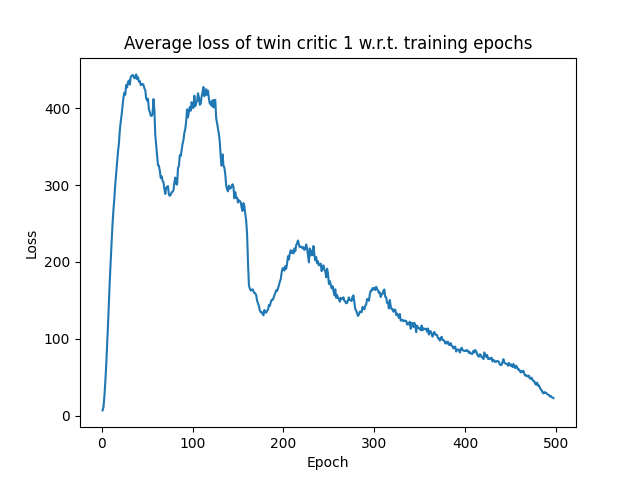
\includegraphics[width=0.6\textwidth]{mujoco_lossq1.png}
        \caption{$Q_1$的损失曲线}
        \label{mujocolossq1} 
        \end{figure}

        \begin{figure}
        \centering
        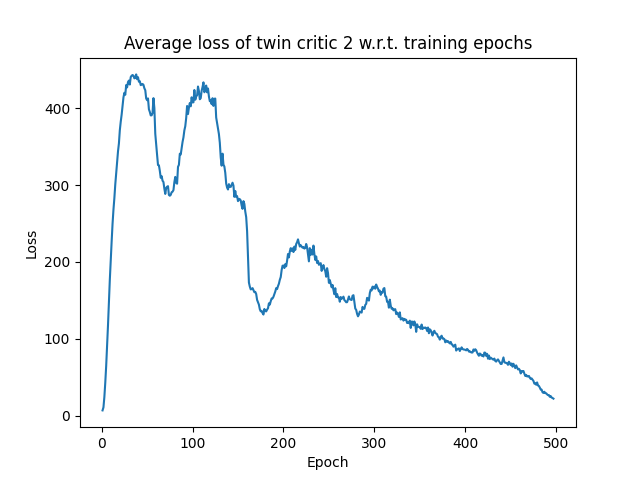
\includegraphics[width=0.6\textwidth]{mujoco_lossq2.png}
        \caption{$Q_2$的损失曲线}
        \label{mujocolossq2} 
        \end{figure}

        每个片段的平均环境奖励如图\ref{mujocoreward}所示。
        可以看出,随着训练的代数增多,环境的奖励开始逐渐增大,最终达到-5左右。
        \begin{figure}
        \centering
        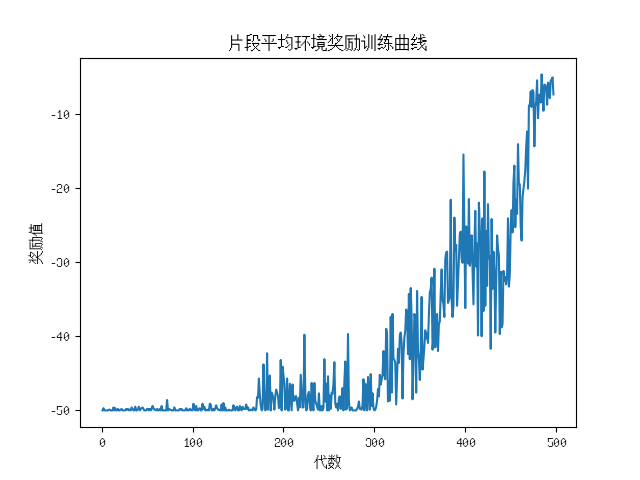
\includegraphics[width=0.6\textwidth]{mujoco_reward.png}
        \caption{环境奖励}
            \label{mujocoreward}
        \end{figure}

        平均每个片段的成功率如图\ref{mujocosuc}所示。
        每个片段的成功与否是通过片段末尾的奖励来判断的,若片段末尾的状态中的已完成的目标与期望目标的距离小于给定值,得到了值为0.0的奖励,就说这个片段成功完成了任务。由于成功率仅仅是10个片段的平均值得到的,因此它只能取到10个离散的值。
        因为成功率的计算只考虑了最后一个状态,所以成功率曲线与平均奖励曲线不完全相同。
        \begin{figure}
        \centering
        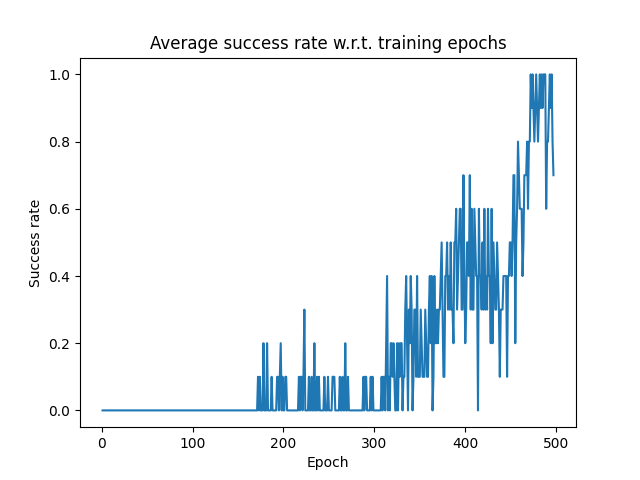
\includegraphics[width=0.6\textwidth]{mujoco_suc_rate.png}
        \caption{任务目标的平均成功率}
            \label{mujocosuc}
        \end{figure}

        在训练完成后,仿真环境\emph{FetchReach-v1}中的这个机械臂已经可以控制它的关节并快速地使末端执行器达到红点位置,成功率约为90\%。如图\ref{mujoco_gym}所示,机械臂成功地完成了任务.
        \begin{figure}
        \centering
        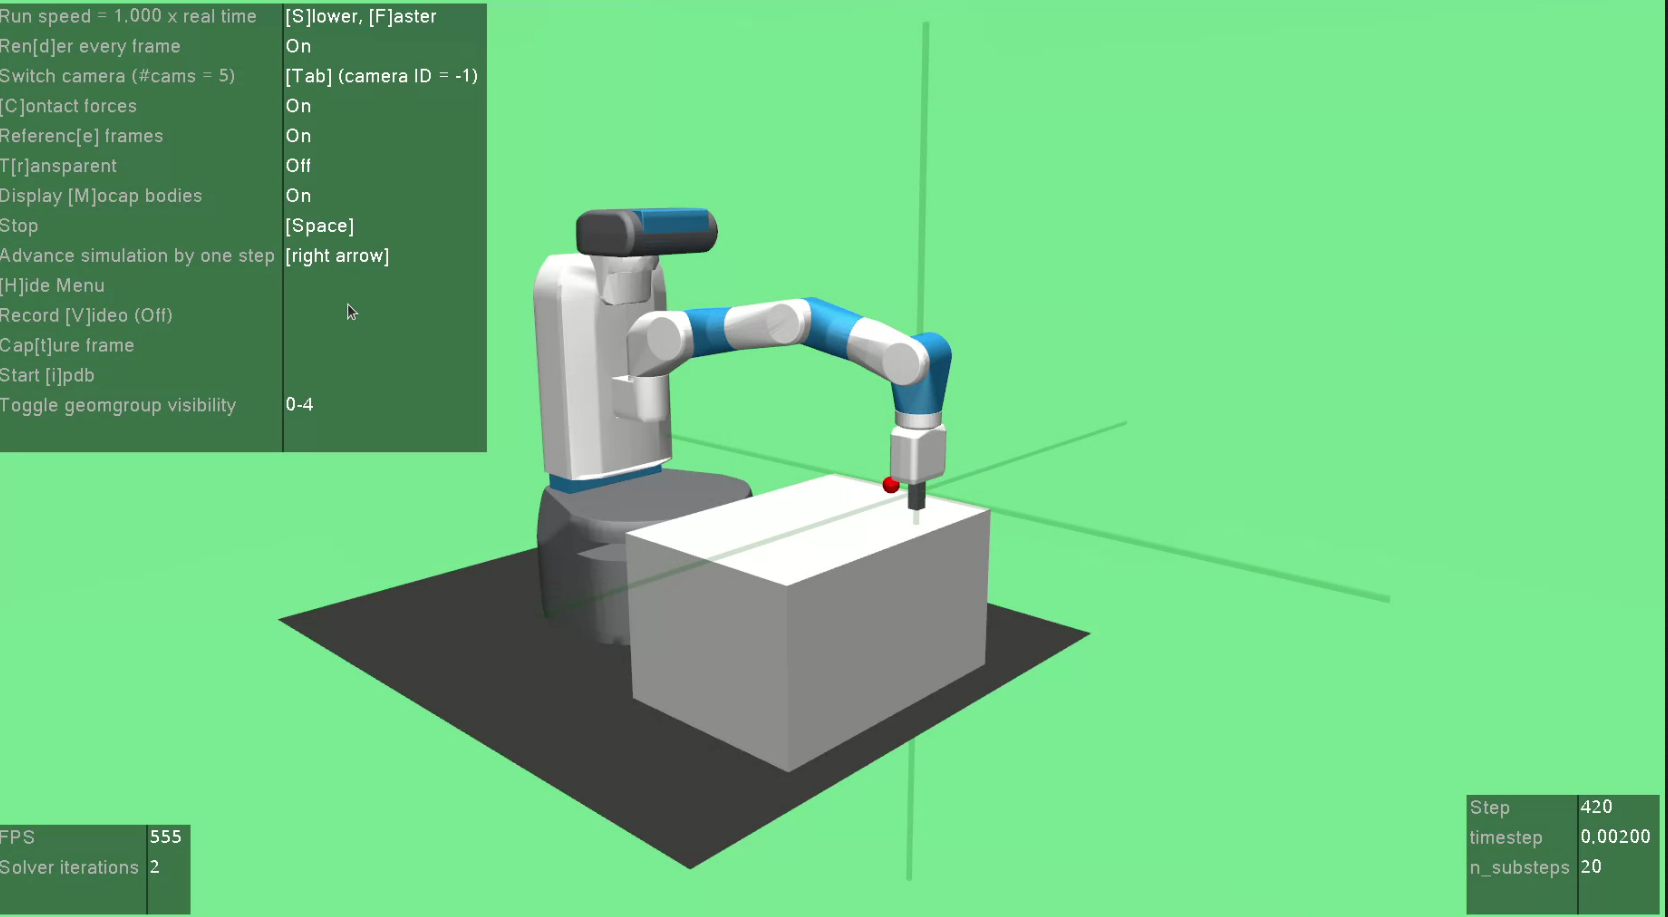
\includegraphics[width=0.8\textwidth]{mujoco_gym.png}
            \caption{Fetch便携机械臂控制关节使末端执行器达到了红点位置,成功完成了指定任务目标。}
            \label{mujoco_gym}
        \end{figure}


